%!xelatex = 'xelatex --halt-on-error %O %S'

\documentclass{buaaemp}
\usepackage{physics}
\usepackage{float}
\newcommand{\SrAtom}{\,\textsuperscript{90}\tup{Sr}\,}
\newcommand{\Yatom}{\,\textsuperscript{90}\tup{Y}\,}	\newcommand{\CsAtom}{\,\textsuperscript{137}\tup{Cs}\,}	\newcommand{\CoAtom}{\,\textsuperscript{60}\tup{Cs}\,}
% \renewcommand{\d}{\mathrm{d}}
% \newcommand{\vb}[1]{\boldsymbol{#1}}
\begin{document}


% 标题,作者
\emptitle{用快速电子验证动量-动能的相对论关系}
\empauthor{智朝晖}{张高龙}

% 奇数页页眉 % 请在这里写出第一作者以及论文题目
\fancyhead[CO]{{\footnotesize 智朝晖: 用快速电子验证动量-动能的相对论关系}}


%%%%%%%%%%%%%%%%%%%%%%%%%%%%%%%%%%%%%%%%%%%%%%%%%%%%%%%%%%%%%%%%
% 关键词 摘要 首页脚注
%%%%%%%%关键词
\Keyword{动量-动能关系,$\beta$衰变,$\beta$粒子,狭义相对论}
\twocolumn[
\begin{@twocolumnfalse}
\maketitle

%%%%%%%%摘要
\begin{empAbstract}
经典力学和电磁学以及光学之间的矛盾,促成了狭义相对论理论的诞生.狭义
相对论理论对于高速物体的运动,和经典力学对于物体的动量-动能关系,给
出了不同的预计.本实验通过测量高能$\beta$粒子的动量和动能,验证了狭
义相对论对于高速运动物体动量-动能关系的预计.并且通过对于空气中$\beta$粒子运动的研究,证明了$\beta$粒子在空气中运动时会损失能量.
\end{empAbstract}

%%%%%%%%首页角注,依次为实验时间、报告时间、学号、email
\empfirstfoot{2022-09-15}{2022-9-16}{20377365}{20377365@buaa.edu.cn}
\end{@twocolumnfalse}
]
%%%%%%%%!首页角注可能与正文重叠,请通过调整正文中第一页的\enlargethispage{-3.3cm}位置手动校准正文底部位置:
%%%%%%%%%%%%%%%%%%%%%%%%%%%%%%%%%%%%%%%%%%%%%%%%%%%%%%%%%%%%%%%%
%  正文由此开始
\wuhao 
%  分栏开始

\section{引~~言}
19世纪,电磁理论得到了极大的发展;麦克斯韦(James C. Maxwell)等人的工作表明,电磁理论可以完美地整合到一组方程中\supercite{maxwell1865dynamical},这便是麦克斯韦方程组。麦克斯韦方程组完整地描述了经典电动力学中的现象,其波动解自然地给出了\textit{电磁波}的预测;通过计算波速:
	\begin{equation}
		c = \frac{1}{\sqrt{\epsilon_0\mu_0}}
		\label{eq:lightSpeed}
	\end{equation}
	麦克斯韦发现\supercite{maxwell1865dynamical}, 可见光正是一种电磁波,从而统一了光学和电磁学。
	
	然而,麦克斯韦方程与经典的伽利略变换不可调和。于是人们猜测,麦克斯韦方程实际只适用于一个特殊的参考系;相应地,电磁波在一种特殊的介质——以太(aether)中传播,可以通过精确测量光速的变动获得地面参考系相对以太的漂移速度。然而,实验迹象表明,这一漂移速度十分微小;迈克尔逊--莫雷实验(Michelson–Morley experiment, 1887)\supercite{michelson1887relative} 给出漂移速度的上限为 \SI{8}{\km/\s}, 考虑地球的公转以及太阳系的运动,这一速度实在微乎其微,令人费解\footnote{%
		最近的实验结果给出的上限为$10^{-17}c \approx \SI{3}{\nm/\s}$, 参见 \cite{herrmann2009rotating}. 
	}。

 \enlargethispage{-3.3cm}
 
	人们不得不转而考虑另一种可能的办法,即对伽利略变换进行修正。经由洛仑兹(Hendrik Lorentz, 参见\cite{lorentz1904electromagnetic})、庞加莱(Henri Poincaré, 参见\cite{poincare1976measure})及爱因斯坦(Albert Einstein)等人的共同努力,以洛仑兹变换为基础的狭义相对论时空观得以建立。相对论时空观与经典时空观的主要差异在于:
	\begin{enumerate}
	\item \textbf{光速不变:}在所有惯性系中,真空光速恒为$c$, 它同时也是运动速度的上限;
	\item \textbf{相对时空:}不存在绝对时空,尤其是不存在绝对的时间坐标;所有惯性系在物理上都是平等的,物理规律具有相同的形式。\vspace{2ex}
	\end{enumerate}

	相对论时空观自然与电动力学相容,但又引出了一些新的疑问。例如,作为时间相对性的直接推论,运动的时钟与静止的时钟并不同步(\textit{钟慢效应});类似的反直观现象还有\textit{动尺收缩}等等。进一步,对于高速运动的粒子而言,狭义相对论的动力学对物体的动量--动能关系做出了不寻常的预计;通过探测高速运动粒子的动量和能量,我们可以方便地验证这一新的\textit{色散关系}(dispersion relation, 借用了光学中动量--能量关系的等价表述),从而初步检验狭义相对论的正确性;此即本实验的首要目的。
\section{理论}

	相对论性的时空由事件(events)构成,时空间隔表示为\textit{四矢量}:
	\begin{equation}
        \begin{gathered}
        \dd{x^\mu} \sim
	   \pqty{\begin{smallmatrix}
		c\,\dd{t} \\[1ex] \dd{\vb{x}}
		\end{smallmatrix}}, \mu = 0,1,2,3  \\
	\dd{x^0}  = c\dd{t},  \dd{x^i} = \dd{\vb{x}^i}, 
		i=1,2,3
            
        \end{gathered}
	\end{equation}
 
	其中$c$为光速;光速不变原理表明,变换到另一惯性系后,相应的\textbf{时空间隔}保持不变(类似于洛仑兹变换中,空间间隔保持不变),即:
	\begin{equation}
	\begin{gathered}
		\eta_{\mu\nu} \dd{x^\mu} \dd{x^\nu}
		\equiv \sum_{\mu,\nu} \eta_{\mu\nu} \dd{x^\mu} \dd{x^\nu}  \\
		= (c\dd{t})^2 - \dd{\vb{x}}^2\ 
		\textit{是洛仑兹不变量(标量),} \\
		\eta_{\mu\nu} \sim
		\pqty{\begin{smallmatrix}
			1 & & & \\
			& -1 & & \\
			& & -1 & \\
			& & & -1
		\end{smallmatrix}}
	\end{gathered}
	\end{equation}
	
	考察运动物体的\textit{共动}参考系,其时间坐标$\tau$称为\textit{固有时}或\textit{原时},有:
	\begin{equation}
	\begin{gathered}
		(c\dd{\tau})^2 - 0 = (c\dd{t})^2 - (\dd{\vb{x}})^2 \\
		\Rightarrow\quad
		\dd{\tau} = \dd{t} \sqrt{1 - \frac{\vb{v}^2}{c^2}}
		= \frac{1}{\gamma}\dd{t},\\
	\end{gathered}
	\end{equation}
	这里$\gamma = \frac{1}{\sqrt{1 - \frac{\vb{v}^2}{c^2}}}$. $\gamma$因子表征了相对论与经典情形的差异。
	
	四动量$p^\mu = m\dv{x^\mu}{\tau} \sim \gamma m
		\pqty{\begin{smallmatrix}
			c \\[1ex] \vb{v}
		\end{smallmatrix}}
		=
		\pqty{\begin{smallmatrix}
			E/c \\[1ex] \vb{p}
		\end{smallmatrix}}$, 它同样是洛仑兹标量;这给出:
	\begin{equation}
	\begin{gathered}
		\eta_{\mu\nu} p^\mu p^\nu
		= \pqty{\frac{E}{c}}^2 - \vb{p}^2 = (mc)^2,\\
		E^2 = \vb{p}^2 c^2 + m^2 c^4
		\label{eq:E-Prelations}
	\end{gathered}
	\end{equation}
	此即相对论性色散关系。我们发现,非零质量的粒子不仅具有动能,还具有\textit{静能}$mc^2$; 扣除掉静能后,粒子的动能可表示为:
	\begin{equation}
        \begin{gathered}
            E_k = \sqrt{p^2 c^2 + m^2 c^4} - m^2 c^4 \\ 
        \to \frac{1}{2} mv^2 
        \pqty{1 + \mcal{O}\,\pqty{\frac{v}{c}}^2}
        \label{eq:relativityEk}
        \end{gathered}
	\end{equation}
	
	可见,在低速极限下,相对论性色散关系回归至经典情形;而对于高速运动的粒子,$\pqty{\frac{v}{c}}^2$阶项不可忽略,两者将会出现显著的差异。本实验即采用$\beta$衰变产生的高速$\beta$粒子,试图观测这一非经典的现象。
 
\section{实~~验}
\subsection{实验原理}
实验装置的基本结构如图 \ref{fig:app} 所示,
	使用\SrAtom--\Yatom\,$\beta$源产生高速$\beta$粒子(负电子,质量$m = \SI{.511}{\MeV/c^2}$),能量上限为 \SI{2.27}{\MeV}, 假定相对论色散关系确切无误,这意味着粒子的速度最高可达 97\% 光速,应当出现显著的相对论效应。
	
	带电粒子的动量通过\textbf{磁谱仪}测定。据经典电动力学,磁场中电子的运动方程:
	\begin{equation}
		\dv{\vb{p}}{t} = -e\vb{v}\times\vb{B}
	\end{equation}
	注意到相对论与电动力学的相容性,此运动方程对高速情形依然成立;垂直射入匀强磁场中的粒子轨迹为圆弧,方程进一步简化为:
	\begin{equation}
		p = eBR = \pqty{\frac{BRc}{\si{M\V}}} \frac{\si{\MeV}}{c}
	\end{equation}
	
	\begin{figure}[!h]
	\vspace{-3ex}
	\centering
	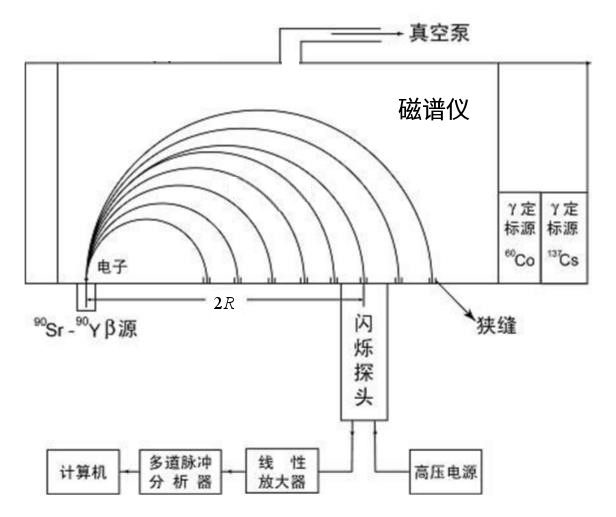
\includegraphics[width=.6\linewidth]{image/app+.png}
	\caption[装置]{实验装置示意图,参考\cite{钱建强2016近代物理实验}. 
		\vspace{-.5ex}}
	\raggedright\small
	\textit{\hphantom{说明}
		$\beta$粒子源出射的粒子经准直后进入磁谱仪,
		真空泵可控制其真空度,减少碰撞导致的能动量改变。
		$\beta$粒子运动半周后离开磁谱仪,进入闪烁探头;
		数据按图示流程进行采集、分析。闪烁探头固定在轨道上,有坐标$x$便于确定其位置;实际有:\vspace{-1.2ex}
		\[2R = x - \SI{10}{\cm}\]}
	\vspace{-2ex}
	\label{fig:app}
	\end{figure}
	
	应当注意,辐射阻尼可能导致粒子损失动能。利用亚伯拉罕--洛仑兹方程:
	\begin{equation}
		\vb{F} = \frac{e^2}{6\pi\epsilon_0 c^3} \dot{\vb{a}}
	\end{equation}
	结合本实验中装置的$B = \SI{636.6}{G} = \SI{63.66}{\milli\tesla}$, 加速度的变化率$\dot{a} \sim \frac{v^2}{r} \cdot \frac{v}{r}$, 估计辐射阻尼的等效作用力$F$及外磁场作用力$evB$分别为:
	\begin{equation}
		F \sim \frac{e^2}{6\pi\epsilon_0 r^2}
			\pqty{\frac{v}{c}}^3
			\sim \SI{e-26}{\N},\\
		evB \sim ecB \pqty{\frac{v}{c}}
			\sim \SI{e-12}{\N}
	\end{equation}
	因此可以安全地略去辐射阻尼的影响。
	
	动能测定通过 NaI (Tl) \textbf{闪烁体探测器}实现。入射粒子的动能传递给闪烁体使之激发、退激,放出光子(\textit{闪烁}),经光电倍增、前置放大、线性放大等步骤,转化为充分强的电脉冲输入\textbf{多道分析器};多道分析器将脉冲强度转化为道址$n$存储并计数。
	
	注意,上述能量转换过程基本上是线性的,即有$n\propto E$; 利用标准放射源\CsAtom 和\CoAtom 进行定标,可进一步确定$n$--$E$关系,由此获得粒子的动能。此外,$\beta$粒子在穿入、穿出真空室以及进入探头的过程中存在能量损失,需要进行修正;采用 \cite{钱建强2016近代物理实验} 给出的数值进行修正\footnote{%
		参考\cite{钱建强2016近代物理实验} p.\numrange{109}{110}, 表4.1-1及4.1-2. }。


\subsection{实验数据}
最后的实验结果如下

\begin{table}[h]
\begin{tabular}{lllll}
能量/MeV & 0.184 & 0.662 & 1.17 & 1.33 \\ 
道数/CH  & 97    & 313   & 536  & 605          
\end{tabular}
\caption{测量的道数对应的能量}
\label{tab:measure}
\end{table}

利用最小二乘法,拟合出来能量$E$和道数$CH$的关系为:
\begin{equation}
\begin{gathered}
     E=a+b\times CH \\
    \to E=0.0023CH-0.0383, R^=0.9999
\end{gathered}
\end{equation}

\begin{table}[h]
\begin{tabular}{llllll}
x & x\_1 & x\_2 & x\_3 & x\_4 & x\_5 \\ 
位置/cm &12 &14 &16 &18 &20 \\
CH  & 300  & 370  & 457  & 535  & 620 \\
动量 & 1.142 &1.332 &1.523 & 1.713 & 1.903 \\
能量 &0.6517 &0.8127 &1.0128 &1.1922 &1.3877

\end{tabular}
\caption{不同位置的粒子对应的道数和动量,以及道数对应的能量}
\label{tab:beta}
\end{table}

\section{实验结果与分析}
根据\ref{eq:relativityEk}$E_k = \sqrt{p^2 c^2 + m^2 c^4} - m^2 c^4$我们带入得到动能的理论值为\ref{tab:my_label}:

\pagebreak
结果如图\ref{fig:my_label}所示:

\begin{figure}[htbp]
    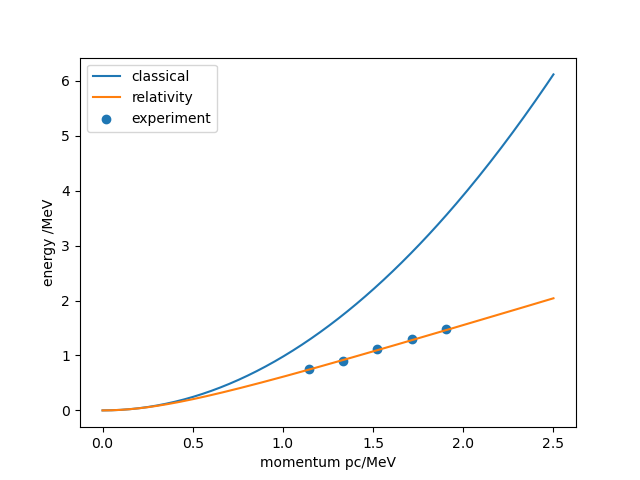
\includegraphics[width=0.4\textwidth]{image/betaray.png}
    \caption{粒子的相对论和经典动能动量关系以及实验数据}
    \label{fig:my_label}
\end{figure}


\begin{table}[h]
    \centering
    \begin{tabular}{llllll}
         理论值 &0.740 & 0.916 &1.096 &1.277 &1.459  \\
         测量值 &0.6517 &0.8127 &1.0128 &1.1922 &1.3877 \\
         真实值 &0.749 &0.9007 &1.109 &1.2986 &1.485
    \end{tabular}
    \caption{能量的理论值、测量值、真实值}
    \label{tab:my_label}
\end{table}

我们可以看到相对误差为:1.2\%, 1.63\%, 1.24\%, 1.72\%, 1.75\%.误差很小。




在此基础上,我们尝试估计$\beta$粒子在$\SI{1}{atm}$的\textit{衰减长度}$L_0$. 与空气分子的碰撞导致沿轨迹运动的粒子数目指数衰减,考虑探测装置的效率$\epsilon$, 有探测到的粒子数目:
	\begin{equation}
		N_0 = \epsilon C\,e^{-\frac{L}{L_0}},\quad
		p = p_0 = \SI{1}{atm}
	\end{equation}
	
	此外,粒子的自由程反比于压强,故改变压强$p$时,有:
	\begin{equation}
		N = \epsilon C\,e^{-\frac{pL}{p_0 L_0}}\quad
		\Longrightarrow\quad
		L_0 = L\pqty{1 - \frac{p}{p_0}} \bigg/ \ln\frac{N}{N_0}
	\end{equation}
	本实验中,$L = \pi R,\,\pqty\big{1 - \frac{p}{p_0}} \to 1$, 进一步有:
	\begin{equation}
		L_0 = \pi R \bigg/ \ln\frac{N}{N_0}
	\end{equation}

 $\beta$粒子在空气中的衰减长度$L_0$大致为三十几厘米,且$L_0$似乎随着粒子能动量的增大而增大。可以肯定的是,该能量范围的$\beta$粒子在 \SI{1}{atm} 下的衰减长度大致均在 \SIrange{30}{40}{cm} 上下,与$L$在同一量级。这也进一步肯定了在真空环境中进行实验的必要性。
\section{结~~论}
实验证实了高能$\beta$粒子的动量--动能的关系(色散关系)满足狭义相对论的理论预测,即在误差容许的范围内,有:
	\begin{equation}
		E_k = \sqrt{p^2 c^2 + m^2 c^4} - m^2 c^4
		\tag{\ref{eq:relativityEk}}
	\end{equation}
	从而初步验证了狭义相对论对高速运动物体的适用性。同时,实验结果与经典理论的严重偏离确认了经典力学对高速运动不适用。
	
	在此基础上,实验估测了$\beta$粒子在 \SI{1}{atm} 空气中的衰减长度$L_0 \sim \SIrange{30}{40}{cm}$, 从而强调了真空环境对提高数据质量的重要意义。


%%%%%%%%%%%%%%%%%%%%%%%%%%%%%%%%%%%%%%%%%%%%%%%%%%%%%%%%%%%%%%%%
%  参考文献
%%%%%%%%%%%%%%%%%%%%%%%%%%%%%%%%%%%%%%%%%%%%%%%%%%%%%%%%%%%%%%%%
%  参考文献按GB/T 7714-2015《文后参考文献著录规则》的要求著录. 
%  参考文献在正文中的引用方法:\cite{bib文件条目的第一行}

\renewcommand\refname{\heiti\wuhao\centerline{参考文献}\global\def\refname{参考文献}}
\vskip 12pt

\let\OLDthebibliography\thebibliography
\renewcommand\thebibliography[1]{
  \OLDthebibliography{#1}
  \setlength{\parskip}{0pt}
  \setlength{\itemsep}{0pt plus 0.3ex}
}

{
\renewcommand{\baselinestretch}{0.9}
\liuhao
\bibliographystyle{gbt7714-numerical}
\bibliography{./TempExample}
}


\end{document}
